\documentclass[10pt,a4paper]{article}
\usepackage[utf8]{inputenc} % para poder usar tildes en archivos UTF-8
\usepackage[spanish]{babel} % para que comandos como \today den el resultado en castellano
\usepackage{a4wide} % márgenes un poco más anchos que lo usual
\usepackage{caratula}
% \usepackage[left=3cm,right=3cm,bottom=3cm,top=3cm]{geometry}

% Comandos para formato
\usepackage[table,xcdraw]{xcolor}
\usepackage{hyperref}

% Comandos para simbolos matematicos.
\usepackage{amsmath, amssymb, tabularx}

% Comandos para referencias
\usepackage{natbib}

% Comandos para Figuras, Graficos, Tikz etc.
\usepackage{tikz}
\usepackage{epsfig}
%\usepackage{pgfplots}
\usepackage{graphicx}
\usepackage{epsfig}
\usepackage{caption}
\usepackage{subcaption}
\usepackage{svg}

% Comandos para teoremas etc.
\usepackage{amsthm}
\newtheorem{theorem}{Teorema}
\newtheorem{lemma}[theorem]{Lema}
\newtheorem{proposition}[theorem]{Proposición}
\newtheorem{remark}{Observación}
\newtheorem{corollary}{Corolario}
% \newproof{proof}{Demostración}

% Comandos para algoritmos.
\usepackage[noend]{algpseudocode}
\usepackage{algorithm}
\algnewcommand{\IfThenElse}[3]{% \IfThenElse{<if>}{<then>}{<else>}
\State \algorithmicif\ #1\ \algorithmicthen\ #2\ \algorithmicelse\ #3}
\algnewcommand{\IfThen}[2]{% \IfThenElse{<if>}{<then>}
\State \algorithmicif\ #1\ \algorithmicthen\ #2}
\renewcommand{\algorithmicrequire}{\textbf{Input:}}
\renewcommand{\algorithmicensure}{\textbf{Output:}}

\begin{document}

\titulo{TP 1: Eliminación Gaussiana, \\ Matrices Tridiagonales y Difusión}
\materia{Métodos Numéricos}

\integrante{Asmad, Victor}{760/19}{vasmad@dc.uba.ar}
\integrante{Lopez Luque, Matías}{192/14}{matimatote@gmail.com}
\integrante{Romano, Germán}{786/11}{romano.german17@gmail.com}

\maketitle

\newpage

\tableofcontents

\newpage

%%%%%%%%%%%%%%%%%%%%%%%%%%%%%%%%%%%%%%%%%%%%%%
\section{Resumen} \label{sec:Resumen} El objetivo de este trabajo es desarrollar diferentes métodos de resolución de sistemas de ecuaciones basados en el algoritmo de Eliminación Gaussiana, y experimentar y evaluar su performance, tanto en tiempo como en precisión, al aplicarlos al modelado de un problema de difusión. Se hace foco principalmente en sistemas de ecuaciones tridiagonales, cuyas características particulares son aprovechadas para mejorar la performance de la solución propuesta.

\bigbreak

\textbf{Palabras Clave:} Matrices, Eliminación Gaussiana, Sistemas tridiagonales, Laplaciano Discreto, Difusión

%%%%%%%%%%%%%%%%%%%%%%%%%%%%%%%%%%%%%%%%%%%%%%
\section{Introducción} \label{sec:Intro}

\subsection{Sistemas de ecuaciones} \label{intro_sistemas_ecuaciones}
Un sistema de $n$ ecuaciones con $n$ incógnitas puede escribirse de forma matricial como $Ax\ =\ b$, siendo $A \in \mathbb{R}^{n \times n}$ la matriz cuadrada con los coeficientes de las incógnitas, $x \in \mathbb{R}^{n \times 1}$ el vector de incógnitas y $b \in \mathbb{R}^{n \times 1}$ el vector con los coeficientes independientes. Concatenando el vector $b$ a derecha de la matriz $A$ obtenemos la matriz aumentada $A^{\prime} \in \mathbb{R}^{n \times n+1}$.

Los sistemas de ecuaciones con una única solución pueden ser resueltos mediante el algoritmo de Eliminación Gaussiana \cite{burden-gauss} con una complejidad computacional de orden $\mathcal{O}(n^3)$. Este toma como input la matriz aumentada $A^{\prime}$ y en cada paso procede a anular los elementos por debajo de la diagonal de cada columna mediante operaciones de fila, siempre que sea posible, obteniendo como resultado una matriz escalonada. El elemento ubicado en la diagonal de la matriz que se utiliza en cada paso como base de las operaciones se llama pivot. Por último, se despejan y reemplazan hacia atrás cada una de las incógnitas.

Uno de los casos en que el algoritmo no es capaz de devolver una solución es cuando, en alguno de los pasos, se halla un elemento nulo en la diagonal. En estos casos puede aplicarse pivoteo parcial o total, consistente en permutar filas y/o columnas para desbloquear el paso y continuar con el procedimiento. El pivoteo permite también reducir el error numérico de la resolución, al optar en cada paso por el mayor elemento de la matriz a modo de pivot.

\subsection{Sistemas tridiagonales} \label{intro_sistemas_tridiagonales}
Un tipo particular de matrices ralas, cuyos elementos son mayormente nulos, son las llamadas tridiagonales. Estas contienen elementos nulos por fuera de la diagonal principal y las diagonales adyacentes por encima y por debajo de la principal. Un sistema de ecuaciones tridiagonal y su matriz asociada tienen la forma:

\begin{equation} \label{eq:tridiagonal}
	a_{i} x_{i-1} + b_{i} x_{i} + c_{i} x_{i+1} = d_{i}
\end{equation}


\[
\begin{bmatrix}
b_{1} & c_{1} &  &  & 0 \\
a_{2} & b_{2} & c_{2} &  &  \\
 & a_{3} & b_{3} & \ddots &  \\
 &  & \ddots & \ddots & c_{n-1} \\
0 &  &  & a_{n} & b_{n} \\
\end{bmatrix}
\begin{bmatrix}
x_{1} \\
x_{2} \\
x_{3} \\
\vdots \\
x_{n} \\
\end{bmatrix}
=
\begin{bmatrix}
d_{1} \\
d_{2} \\
d_{3} \\
\vdots \\
d_{n} \\
\end{bmatrix}
\]

En estos casos, el sistema puede representarse mediante sólo 4 vectores $a$, $b$, $c$ y $d$ de largo $n$ (siendo nulos $a_{1}$ y $c_{n}$). Aprovechando esto, puede desarrollarse una versión del algoritmo de Eliminación Gaussiana que omite las operaciones triviales correspondientes a la gran cantidad de elementos nulos de la matriz y reduce la complejidad computacional al orden $\mathcal{O}(n)$. Para los casos en que se opere múltiples veces con la misma matriz $A$ para diferentes vectores $d$, también se puede hacer un pre-cómputo de la Eliminación Gaussiana de $A$ por única vez para luego aplicarlo sobre los vectores $d$, reduciendo aún más la cantidad total de operaciones a realizar.


\subsection{Laplaciano discreto} \label{intro_laplaciano_discreto}
Un caso de aplicación de sistemas tridiagonales a procesamiento de grafos e imágenes es el cálculo del operador de Laplace o Laplaciano en su versión discreta. Para el caso unidimensional la operación está dada por:

\begin{equation} \label{eq:laplaciano}
	u_{i-1} - 2u_{i} + u_{i+1} = d_{i}
\end{equation}

siendo $u_{-1} = u_{n} = 0$. El sistema en forma matricial tiene la forma:

\[
\begin{bmatrix}
-2 & 1 &  &  & 0 \\
1 & -2 & 1 &  &  \\
 & 1 & -2 & \ddots &  \\
 &  & \ddots & \ddots & 1 \\
0 &  &  & 1 & -2 \\
\end{bmatrix} 
\begin{bmatrix}
u_{1} \\
u_{2} \\
u_{3} \\
\vdots \\
u_{n} \\
\end{bmatrix}
=
\begin{bmatrix}
d_{1} \\
d_{2} \\
d_{3} \\
\vdots \\
d_{n} \\
\end{bmatrix}
\]

Aprovechando el sistema matricial tridiagonal asociado al problema, puede aprovecharse la adaptación de Eliminación Gaussiana para sistemas tridiagonales para hallar el vector $u$ asociado a cada vector $d$.

\subsection{Difusión} \label{intro_difusion}
Este tipo de sistemas de ecuaciones también encuentra aplicación en el modelado de procesos estocásticos de difusión, donde una entidad se difunde típicamente
desde un lugar de mayor concentración hacia uno de menos. Es posible estudiar la evolución promedio de una densidad de partículas inicial resolviendo la ecuación de difusión de forma discreta
mediante Eliminación Gaussiana para sistemas tridiagonales \cite{langtangen-difusion}.

A partir de un vector inicial $u^{(0)}$ con magnitudes positivas, para cada punto discreto $i$, $u_{i}$ se atenuará y se dispersará hacia $u_{i-1}$ y $u_{i+1}$. En pos de mantener constante la suma total (es decir, la magnitud), la operación a utilizar deberá mantener iguales los ritmos de dispersión y atenuación. El operador laplaciano garantiza la conservación puesto que la suma de sus coeficientes es $1 - 2 + 1 = 0$. Considerando el incremento para el paso $k$ como una
fracción $\alpha$ del operador laplaciano de $u_{k}$, la ecuación resultante tiene la forma

\begin{equation} \label{eq:difusion}
	u_{i}^{(k)} - u_{i}^{(k-1)} = \alpha (u_{i-1}^{(k)} - 2 u_{i}^{(k)} + u_{i+1}^{(k)})
\end{equation}

En forma matricial, el sistema se puede expresar como $A u^{(k)} = u^{(k-1)}$. Resolviendo el sistema de forma iterativa, se obtiene la
evolución del vector u para $k = \{1, 2, 3, ..., m\}$. El resultado obtenido equivale a simular infinitas trayectorias individuales y analizar cómo se
distribuyen en promedio.

%%%%%%%%%%%%%%%%%%%%%%%%%%%%%%%%%%%%%%%%%%%%%%
\section{Desarrollo} \label{sec:Desarrollo}

\subsection{Eliminación Gaussiana sin pivoteo} \label{desarrollo_gauss_sin_pivoteo}
Dada una matriz $A \in \mathbb{R}^{n \times n}$ y un vector de términos independientes $b \in \mathbb{R}^{n}$, el algoritmo de eliminación gaussiana consta de dos etapas.

\subsubsection*{Diagonalización}

La primera etapa consiste en recorrer las filas de arriba hacia abajo. Para cada fila $i$ se utiliza el elemento $a_{ii}$ como pivot. A continuación, se busca llevar a 0 a todos los elementos $a_{ji}$ con $i < j \leq n$. Para esto se le resta a cada fila $j$ un múltiplo de la fila $i$, es decir que para cada $k$, $1 \leq k \leq n$, se hace la asignación $a_{jk} = a_{jk} - \frac{a_{ji}}{a_{ii}} * a_{ik}$. De esta manera, al elemento $a_{ji}$ se le asigna $a_{ji} - \frac{a_{ji}}{a_{ii}} * a_{ii} = a_{ji} - a_{ji} = 0$. De forma simultanea, se aplica la misma operación en el vector independiente $b$, haciendo la asignación $b_{j} = b_{j} - \frac{a_{ji}}{a_{ii}} * b_{i}$. Esto preserva la equivalencia entre el sistema de ecuaciones original y el resultante del proceso de diagonalización.

El invariante de esta etapa del algoritmo es entonces que, después del $i$-esimo paso, todas las filas $k$ con $i < k \leq n$ tendrán el elemento $a_{ki} = 0$. Una vez finalizada la etapa de diagonalización tendremos una matriz triangular superior y un vector de términos independientes equivalentes al sistema de ecuaciones original.


\begin{algorithm}
    \caption{Diagonalización}\label{alg:diagonalize}
    \begin{algorithmic}
        \Require{$A, b, i$}
        \Ensure{$A, b$}
        \If{$A_{ii} = 0$}
        \State \textbf{exception:} $"$EG no aplicable$"$
        \EndIf
        \For{$j \gets i + 1$ to $n$}
        \If{$A_{ji} \neq 0$}
        \State $escalar \gets \frac{A_{ji}}{A_{ii}}$
        \State $b_{j} \gets b_{j} - escalar * b_{i}$
        \For{$k \gets 1$ to $n$}
        \State $A_{jk} \gets A_{jk} - (A_{ik} * escalar)$
        \EndFor
        \EndIf
        \EndFor
    \end{algorithmic}
\end{algorithm}


\subsubsection*{Sustitución hacia atrás}

Llamemos $A^{1} \in \mathbb{R}^{n \times n}$ a la matriz triangular superior y $b^{1} \in \mathbb{R}^{n}$ al vector de términos independientes resultantes del paso de diagonalización.

La ultima fila de la matriz representa la ecuación $a^{1}_{nn} * x_{n} = b^{1}_{n}$, ya que el resto de los elementos de la fila son $0$. Esta ecuación tiene una única solución $x_{n} = \frac{b^{1}_{n}}{a^{1}_{nn}}$. El método de sustitución hacia atrás consiste en tomar el valor para $x_{n}$ mencionado, y utilizarlo para despejar $x_{n-1}$ en la ecuación de la fila $n - 1$. La ecuación despejada queda entonces $x_{n - 1} = \frac{b^{1}_{n - 1} - (b^{1}_{n} * x_{n})}{a^{1}_{n-1n-1}}$.

Este proceso se repite para todas las ecuaciones restantes, sustituyendo las soluciones obtenidas hasta el momento y despejando la $i$-esima incognita.

\begin{algorithm}
    \caption{Sustitución hacia atrás}\label{alg:backwards-substitution}
    \begin{algorithmic}
        \Require{$A, b$}
        \Ensure{$x$}
        \For{$i \gets n$ to $1$}
        \State $sum \gets 0$
        \For{$j \gets i + 1$ to $n$}
        \State $sum \gets sum + A_{ij} * x_{j}$
        \EndFor
        \If{$A_{ii} \neq 0$}
        \State $x_{i} \gets \frac{(b_{i} - sum)}{A_{ii}}$
        \Else
        \State $x_{i} \gets 0$ \Comment{En este caso el sistema tiene infinitas soluciones}
        \EndIf
        \EndFor
    \end{algorithmic}
\end{algorithm}

\subsubsection*{Algoritmo completo}

Una vez definidos los algoritmos para diagonalización(\ref{alg:diagonalize}) y sustitución hacia atrás (\ref{alg:backwards-substitution}), el algoritmo completo de eliminación gaussiana consiste en realizar el paso de diagonalización para cada una de las filas, y luego llamar al algoritmo de sustitución para la matriz $A^{1}$ y el vector $b^{1}$ modificados.

\begin{algorithm}
    \caption{Eliminación gaussiana}\label{alg:gauss}
    \begin{algorithmic}
        \Require{$A, b$}
        \Ensure{$x$}
        \For{$i \gets 1$ to $n$}
        \State $A, b \gets Diagonalizacion(A, b, i)$ \Comment{Algoritmo \ref{alg:diagonalize}}
        \EndFor
        \State $x \gets Sustitucion(A,b)$ \Comment{Algoritmo \ref{alg:backwards-substitution}}
    \end{algorithmic}
\end{algorithm}

Este algoritmo tiene complejidad temporal de $O(n^{3})$. Para cada una de las $n$ filas se diagonalizan todas las filas inferiores, por lo que se incurren $O(n^{2})$ operaciones entre filas. Cada operación entre filas es del orden $O(n)$, pues se realizan operaciones aritméticas sobre todas sus $n$ columnas.


\subsection{Eliminación Gaussiana con pivoteo} \label{desarrollo_gauss_con_pivoteo}
Como se menciona en \ref{intro_sistemas_ecuaciones}, el algoritmo de eliminación gaussiana explicitado en la sección \ref{desarrollo_gauss_sin_pivoteo} tiene dos problemas. En el paso de diagonalización(\ref{alg:diagonalize}) se define un escalar de la forma $\frac{A_{ji}}{A_{ii}}$ para $1 \leq i \leq n$ y $i < j \leq n$. Si el elemento $a_{ii}$ de la matriz $A$ es $0$, el algoritmo no puede resolver el sistema de ecuaciones.

Otro problema que surge es que si en algún elemento de la diagonal $a_{ii}$ se presenta un valor cercano a $0$, entonces el escalar $\frac{a_{ji}}{a_{ii}}$ tiene el potencial de introducir error numérico a los resultados. Esto se debe a que el resultado de dividir por un valor cercano a $0$ es potencialmente un numero muy elevado, y estos números están más esparcidos en las representaciones de punto flotante.

\smallbreak

Ambos problemas pueden mitigarse modificando el algoritmo de eliminación gaussiana para realizar pivoteo parcial. El pivoteo consiste en, en el paso $i$, $1 \leq i \leq n$, en vez de utilizar el elemento $a_{ii}$ como pivot, permutar la fila $i$ por la fila $j$, con $i < j \leq n$, donde el valor de $a_{ji}$ es el mayor valor de la columna $i$ para las filas entre $i$ y $n$. Los mismos indices deben permutarse en el vector de términos independientes.

\smallbreak

Si ningún valor en la columna $i$ es distinto a $0$, esto significa que $a_{ji} = 0$ para todo $i \leq j \leq n$, es decir que el paso $i$ de diagonalización puede saltearse. El problema de error numérico solo puede mitigarse, ya que dividir por el mayor valor posible genera una menor magnitud de error, pero no puede garantizarse operaciones sin error numérico.

\begin{algorithm}
    \caption{Eliminacion gaussiana con pivoteo}\label{alg:gauss-pivot}
    \begin{algorithmic}
        \Require{$A, b$}
        \Ensure{$x$}
        \For{$i \gets 1$ to $n$}
        \State $pivot \gets i$
        \For{$j \gets i + 1$ to $n$}
        \If{$A_{ji} > A_{ii}$}
        \State $pivot \gets j$
        \EndIf
        \EndFor
        \If{$j \neq i$}
        \State $temp \gets A_{i}$ \Comment{Operacion sobre toda la fila $i$}
        \State $A_{i} \gets A_{j}$
        \State $A_{j} \gets temp$
        \State $temp \gets b_{i}$
        \State $b_{i} \gets b_{j}$
        \State $b_{j} \gets temp$
        \EndIf
        \State $A, b \gets Diagonalizacion(A, b, i)$ \Comment{Algoritmo \ref{alg:diagonalize}}
        \EndFor
        \State $x \gets Sustitucion(A,b)$ \Comment{Algoritmo \ref{alg:backwards-substitution}}
    \end{algorithmic}
\end{algorithm}


\subsection{Eliminación Gaussiana para un sistema tridiagonal} \label{desarrollo_gauss_tridiagonal}
Cuando la matriz asociada al sistema a resolver es tridiagonal, dadas las características de dichas matrices, en cada paso de Eliminación Gaussiana sólo se debe anular el elemento inmediatamente debajo de la diagonal principal, dado que el resto de los elementos debajo de la misma son nulos. Esto puede aprovecharse para reducir significativamente la cantidad de operaciones a realizar.

En el ejemplo de la sección \ref{intro_sistemas_tridiagonales} se observa claramente cómo en el paso 1 de Eliminación Gaussiana sólo debe anularse el elemento $a_{2}$ (asumiendo $b_{1} \neq 0$). Lo mismo ocurre en los pasos siguientes. Esto resulta en que el vector $a$, finalizada la ejecución del algoritmo, termine siendo el vector nulo.

En el mismo ejemplo puede también observarse que los elementos inmediatamente superiores a la diagonal principal (vector $c$) no resultan afectados por los pasos de Eliminación Gaussiana, dado que los elementos superiores de su misma columna son nulos, lo que implica que en cada paso se les reste (o sume) cero.

Por lo tanto, en el $i$-ésimo paso de Eliminación Gaussiana sobre una matriz tridiagonal extendida, sólo deben calcularse los nuevos valores de $b_{i+1}$ y $d_{i+1}$, restándoles el elemento inmediatamente superior multiplicado por el factor $\frac{a_{i+1}}{b_{i}}$ (algoritmo \ref{alg:gauss-tridiagonal}).

\begin{algorithm}[H]
\caption{Eliminación Gaussiana para matrices tridiagonales}\label{alg:gauss-tridiagonal}
\begin{algorithmic}
\Require{$a, b, c, d$} 
\Ensure{$a, b, c, d$} 
\For{$i \gets 1$ to $n-1$}     
    \If{$b_{i} = 0$ } \Comment{Se detectó un elemento nulo en la diagonal}
        \State \textbf{exception:} $"$EG no aplicable$"$ 
    \Else
        \State $m \gets \frac{a_{i+1}}{b_{i}}$
        \State $b_{i+1} \gets b_{i+1} - m * c_{i}$
        \State $d_{i+1} \gets d_{i+1} - m * d_{i}$
        \State $a_{i+1} \gets 0$
    \EndIf
\EndFor
\end{algorithmic}
\end{algorithm}

Antes de aplicar cada paso se analiza la presencia de elementos nulos en la diagonal (vector $b$).

Finalmente, como resultado de escalonar una matriz tridiagonal, se obtiene una matriz que sólo contiene elementos no nulos en la diagonal principal (vector $b$) y en su diagonal inmediatamente superior (vector $c$). Esto también puede aprovecharse para reducir la cantidad de operaciones que requiere la sustitución hacia atrás.

Dado que los únicos coeficientes no nulos se hallan en los vectores $b$ y $c$ resultantes del algoritmo anterior, en el despeje de la $i$-ésima fila de la matriz escalonada sólo intervienen dos variables: $x_{i}$ (la variable a despejar) y $x_{i+1}$ (la variable despejada en el paso anterior); en el caso $i = n$, sólo resta despejar $x_{n}$. En el despeje también interviene el término independiente almacenado en el vector $d$ (algoritmo \ref{alg:gauss-tridiagonal-sustitucion}).

Para ciertas aplicaciones, resulta útil resolver el mismo sistema tridiagonal pero variando los términos independientes de las ecuaciones (vector $d$). En esos casos puede aplicarse un pre-cómputo sobre la matriz tridiagonal que permita luego transformar el vector de términos independientes sin necesidad de volver a escalonar la matriz original, para finalmente ejecutar la sustitución hacia atrás. 

\begin{algorithm}[H]
\caption{Sustitución hacia atrás}\label{alg:gauss-tridiagonal-sustitucion}
\begin{algorithmic}
\Require{$b, c, d$} 
\Ensure{$x$}   \Comment{$x$ es el vector solución del sistema}
\State $x \gets (0, \hdots, 0)$
\For{$i \gets n$ to $1$}     
    \If{$i = n$ }
        \If{$b_{i} = 0$ }
            \If{$d_{i} = 0$}
                \State \textbf{exception:} $"$El sistema tiene infinitas soluciones$"$
            \Else \State \textbf{exception:} $"$El sistema no tiene solución$"$
            \EndIf
        \Else \State $x_{i} \gets \frac{d_{i}}{b_{i}} $
        \EndIf
    \Else
        \State $x_{i} \gets \frac{d_{i} - x_{i+1} * c_{i}}{b_{i}} $ \Comment{$b_{i} \neq 0$ pues EG tuvo que haber finalizado}
    \EndIf
\EndFor
\end{algorithmic}
\end{algorithm}

\begin{algorithm}[H]
\caption{Eliminación Gaussiana para matrices tridiagonales con pre-cómputo}\label{alg:gauss-tridiagonal-con-precomputo}
\begin{algorithmic}
\Require{$a, b, c$} 
\Ensure{$a, b, c, d^{pre}$}   \Comment{$d^{pre}$ contiene el pre-cómputo a aplicar sobre $d$}
\State $d^{pre} \gets (0, \hdots, 0)$
\For{$i \gets 1$ to $n-1$}     
    \If{$b_{i} = 0$} \Comment{Se detectó un elemento nulo en la diagonal}
        \State \textbf{exception:} $"$EG no aplicable$"$ 
    \Else
        \State $m \gets \frac{a_{i+1}}{b_{i}}$
        \State $b_{i+1} \gets b_{i+1} - m * c_{i}$
        \State $d^{pre}_{i+1} \gets m$
        \State $a_{i+1} \gets 0$
    \EndIf

\EndFor
\end{algorithmic}
\end{algorithm}

El algoritmo \ref{alg:gauss-tridiagonal-con-precomputo} es una adaptación del algoritmo de Eliminación Gaussiana para matrices tridiagonales, que en cada paso $i$ almacena el coeficiente $m$ necesario para transformar el término $d_{i}$ de los posibles vectores $d$. El algoritmo \ref{alg:gauss-tridiagonal-precomputo-d} muestra cómo, dado un vector $d$ de términos independientes, se obtiene el resultado de aplicarle a dicho vector los pasos de Eliminación Gaussiana pre-computados. Por último, basta aplicar sustitución hacia atrás (algoritmo \ref{alg:gauss-tridiagonal-sustitucion}) sobre los vectores $b$ y $c$ calculados por el algoritmo \ref{alg:gauss-tridiagonal-con-precomputo} y el vector $d$ obtenido mediante al algoritmo \ref{alg:gauss-tridiagonal-precomputo-d}.

\begin{algorithm}[H]
\caption{Aplicación de pre-cómputo sobre un vector $d$}\label{alg:gauss-tridiagonal-precomputo-d}
\begin{algorithmic}
\Require{$d^{pre}, d$} 
\Ensure{$d$} 
\For{$i \gets 1$ to $n$}     
    \If{$i = 1$ }
        \State \textbf{pass} \Comment{Se conserva el elemento $d_{1}$}
    \Else
        \State $d_{i} \gets d_{i} - (d^{pre}_{i} * d_{i-1}) $
    \EndIf
\EndFor
\end{algorithmic}
\end{algorithm}

Mientras que el algoritmo de Eliminación Gaussiana tradicional requiere una cantidad de operaciones del orden de $\mathcal{O}(n^{3})$ \cite{burden-gauss}, la posibilidad de aprovechar las características de las matrices tridiagonales reduce la cantidad de operaciones requeridas al orden de $\mathcal{O}(n)$, lo cual se hace evidente por el hecho de que cada uno de los pasos de la versión para este tipo de matrices (con y sin pre-cálculo) consiste en un ciclo $for$ que recorre los vectores $a$, $b$, $c$ y $d$ de tamaño $n$.

%%%%%%%%%%%%%%%%%%%%%%%%%%%%%%%%%%%%%%%%%%%%%%
\section{Resultados y discusión} \label{sec:Resultados}

\subsection{Tiempos de ejecución} \label{resultados_tiempos_de_ejecucion}
Al trabajar en una computadora, tenemos un problema de límite de dígitos para representación de números, especialmente si trabajamos con números muy chicos ya que tenemos problemas al momento de realizar operaciones entre ellos.
Un ejemplo de ello es que ciertos números muy cercanos al 0, si bien son distintos de 0, su representación en una computadora hace que dicho valor sea representado como 0 y operaciones como la división pueden terminar indefinidas.
Es por tal motivo que se agregó un valor límite, un $\epsilon$ cercano a 0 que se utilizará para medir este riesgo. Dado un $r$ suficientemente chico, si este se encuentra en el intervalo $-\epsilon < r < \epsilon$, asumimos que el número puede afectar las operaciones a realizar.
Ante esta presencia realizamos una advertencia para saber si nos estamos acercando a valores muy chicos y así poder tomar decisiones sobre nuestras matrices de prueba.

Dicho esto, continuaremos con los experimentos para los distintos algoritmos.
Se realizaron comparaciones entre los algoritmos de las siguientes dos maneras:
\begin{itemize}
   \item Eliminación Gaussiana con Pivoteo (tradicional) y Algoritmo Tridiagonal
   \item Algoritmo tridiagonal y Algoritmo tridiagonal con precómputo
\end{itemize}

Se realizaron pruebas con 3 distintos tipos de matrices:
\begin{itemize}
   \item Random Inversible
   \item Estrictamente Diagonal Dominante
   \item Simétrica Definida Positiva
\end{itemize}

El porque se usan estas matrices deriva en los siguientes puntos:
Las matrices random se escogieron para probar la efectividad de los algoritmos en tiempos de términos de ejecución ya que, al ser arbitrarias, no podemos asegurar que estas tengan alguna estructura que brinde ventaja sobre otras de las matrices aleatorias en las pruebas. A demás, para la ejecución, se aseguró de que a todas las matrices con las que se prueba, se les pudiera aplicar la eliminación gausseana.

Las matrices Estrictamente Diagonal Dominantes cumplen con la propiedad de que, sea A una matriz EDD, $|a_{ii}| > \sum_{j = 1, j \neq i}^n |a_{ij}| \forall i=1\dots n$. Teniendo esto presente y desarrollando los pasos, se obtiene que para el i-ésimo paso, el valor de la diagonal no solo no se anulará, si no que será el máximo en esa iteración provocando así que no haya una necesidad de realizar un pivoteo de la misma, por lo cual se puede seguir aplicando correctamente el algoritmo, ahorrando así un tiempo de ejecución considerable.

Para finalizar, la matriz SDP por una de sus propiedades, se tiene que $A_{ii} > 0 \forall i=1\dots n$. 
Por lo cual, la diagonal no es nula y se puede aplicar el i-ésimo paso de la Eliminación Gaussiana. A su vez, por ser una matriz SDP, esta tiene factorización de Cholesky la cual parte de una factorización LU y por lo tanto, se puede aplicar la Eliminación Gausseana.

Para la comparación entre los algoritmos de Eliminación Gaussiana con Pivoteo y Algoritmo Tridiagonal se construyeron múltiples matrices de distintos tamaños acompañados de sus términos independientes (recordar la forma del sistema: $Ax = b$).
Para cada instancia se ejecutó el algoritmo múltiples veces tomando el mínimo tiempo de ejecución en cada una y se construyeron los gráficos de comparación.

La hipótesis respecto de estos algoritmos es que el Algoritmo Tridiagonal se ejecutará mucho más rápido que el algoritmo de Eliminación Gaussiana con pivoteo. Esto ha de deberse a que mientras en el segundo caso se opera sobre la matriz completa (incluyendo la gran cantidad de elementos nulos), en el primero se opera únicamente sobre las tres diagonales de valores no nulos.

Los resultados son los siguientes:

\begin{figure}[H]
   \centering
   \includesvg[scale=0.4]{graficos/4a-pivot-tridg-random.svg}
   \caption{Comparativa EG con Pivot y Tridiagonal. Matrices Random}
   \label{fig:4b-tridg-pre-random-1}
\end{figure}


Se puede ver en la figura \ref{fig:4b-tridg-pre-random-1} como, efectivamente, la hipótesis se cumple siendo el algoritmo tridiagonal el que mantiene un tiempo de ejecución casi constante mientras que el algoritmo de Eliminación Gaussiana crece de forma cuadrática sobre el tamaño de la matriz. En la figura \ref{fig:fig_con_sin_pre-1} se observa que el tipo de matriz no cambia significativamente ni el tiempo total de cada algoritmo, ni la la comparación de tiempos entre ellos.

\begin{figure}[H]
   \begin{subfigure}{.5\textwidth}
      \centering
      \includesvg[scale=0.4]{graficos/4a-pivot-tridg-edd.svg}
      \caption{Ejecución de EDD}
      \label{fig:4b-tridg-pre-edd-1}
   \end{subfigure}%
   \begin{subfigure}{.5\textwidth}
      \centering
      \includesvg[scale=0.4]{graficos/4a-pivot-tridg-sdp.svg}
      \caption{Ejecución de SDP}
      \label{fig:4b-tridg-pre-sdp-1}
   \end{subfigure}
   \caption{Ejecución SDP}
   \label{fig:fig_con_sin_pre-1}
\end{figure}

Para la comparación de los algoritmos tridiagonal (algoritmo \ref{alg:gauss-tridiagonal}) y tridiagonal con precómputo (algoritmo \ref{alg:gauss-tridiagonal-con-precomputo}) se construyó una matriz aleatoria inversible $A$ de tamaño $5000$x$5000$ y $1000$ vectores de términos independientes $d$, utilizada para observar cuál es la diferencia de tiempo entre uno y otro.
La hipótesis sobre este experimentoes que, si bien ambos algoritmos son $\mathcal{O}(n)$, el que no utiliza precómputo debe triangular la matriz en cada ocasión mientras que el otro sólo debe realizarlo una vez.
Esto debería resultar en una leve diferencia entre el crecimiento de una y otra en términos de tiempo.

\begin{figure}[H]
   \centering
   \includesvg[scale=0.4]{graficos/4b-tridg-sincon-pre-random}
   \caption{Comparativa entre algoritmo con y sin precomputo. Matrices Random}
   \label{fig:4b-tridg-pre-random-2}
\end{figure}

Se puede observar claramente en la figura \ref{fig:4b-tridg-pre-random-2} cómo el algoritmo que utiliza precómputo muestra tiempos de ejecución notablemente menores con respecto al algoritmo que no utiliza precómputo, y cómo ambos crecen de manera lineal. Por lo tanto, la hipótesis se cumple.

\begin{figure}[H]
   \begin{subfigure}{.5\textwidth}
      \centering
      \includesvg[scale=0.4]{graficos/4b-tridg-sincon-pre-EDD}
      \caption{Ejecución de EDD}
      \label{fig:4b-tridg-pre-edd-2}
   \end{subfigure}%
   \begin{subfigure}{.5\textwidth}
      \centering
      \includesvg[scale=0.4]{graficos/4b-tridg-sincon-pre-SDP}
      \caption{Ejecución de SDP}
      \label{fig:4b-tridg-pre-sdp-2}
   \end{subfigure}
   \caption{Ejecución SDP}
   \label{fig:fig_con_sin_pre-2}
\end{figure}

Con respecto a los otros dos tipos de matrices (estrictamente diagonal dominante y simétrica definida positiva, figura \ref{fig:fig_con_sin_pre-2}), en ambos  casos se observan resultados similares a los de la figura anterior. Esto se traduce en que el tipo de matriz no afectaría significativamente el tiempo de ejecución de los algoritmos.
Si bien el método con precómputo ejecuta más rápido, ambos crecen de manera lineal y por ende, todo depende del tamaño de la matriz más que del tipo de esta para estos experimentos.

\subsection{Matriz Laplaciana} \label{resultados_matriz_laplaciana}
La segunda parte del análisis consiste en interpretar los resultados de la ejecución del cálculo de la matriz Laplaciana. Se sabe que, aplicado a un vector, este opera como la derivada segunda del mismo.
Es por tal motivo que resulta de interés ver si, mediante un sistema de ecuaciones lineales, se puede encontrar la función que represente a la ecuación $ (d^{2}/dx^{2})u = d $.
Por tal motivo, se definirán distintos $d$ que nos permitan encontrar la función
$$  d_{i} = \begin{cases}
      0 \\
      4/n \ \textit{si} \ i =  \lfloor n/2 \rfloor + 1
   \end{cases}
$$
$$ d_{i} = 4/n^{2} $$
$$ d_{i} = (-1 + 2i/(n - 1))12/n^{2}$$

Se utilizará un valor de $n = 101$ y se procederá a realizar un gráfico de los resultados con el objetivo de ver las funciones que pueden representar.
El resultado se observa en la figura \ref{fig:difusion}.

\begin{figure}[H]
   \centering
   \includesvg[scale=0.5]{graficos/laplaciana.svg}
   \caption{Derivada segunda de los u para distintos d}
   \label{fig:difusion}
\end{figure}


\subsection{Difusión} \label{resultados_difusion}
Lo último sobre la experimentación es el análisis del modelado de un proceso de difusión.
Como se comentó en la Introducción (sección \ref{intro_difusion}), se construirá una matriz a partir de la fórmula allí dada.
La hipótesis es que, debido a la evolución de los $u_i$ en la fórmula $Au^{(k)} = u^{(k-1)}$ que es la que nos indica los valores, debería ocurrir que si partimos de un vector con valores mayores en el centro e inferiores a los lados, a medida que el proceso evoluciona los valores a los costados deberían comenzar a crecer ya que los valores centrales prestarían un porcentaje de sí mismos a sus vecinos.

Esta evolución se puede ver representada en el heatmap de la figura \ref{fig:heatmap_alpha_1}. Allí se observa cómo al principio hay una aglomeración de valores altos en el centro mientras que, a medida que avanza el proceso de difusión, los valores altos se van dispersando hasta llegar a un punto donde todos los valores son altamente similares.

\begin{figure}[H]   
      \centering
      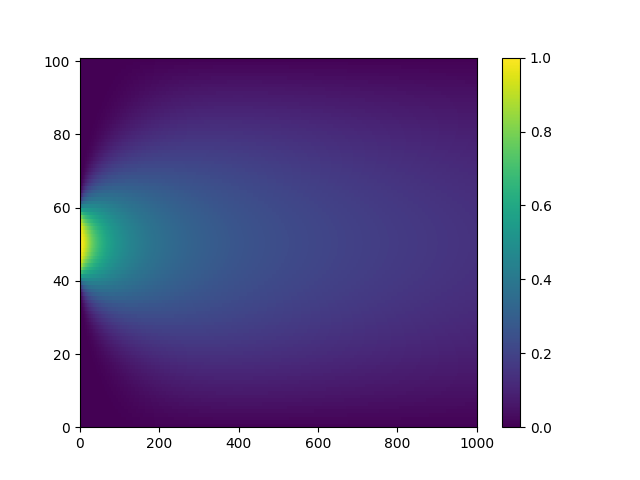
\includegraphics[scale=0.5]{graficos/difusion-alpha1.png}
      \caption{Heatmap para $\alpha = 1$}
      \label{fig:heatmap_alpha_1}
\end{figure}

Si variamos el $\alpha$ y se colocan otros valores como $\alpha = 0.1$ o $\alpha = 10$, se obtienen los resultados presentados en la figura \ref{fig:heatmap_diff_alpha}.

\begin{figure}[H]
      \centering
      \begin{subfigure}{.5\textwidth}
            \centering
            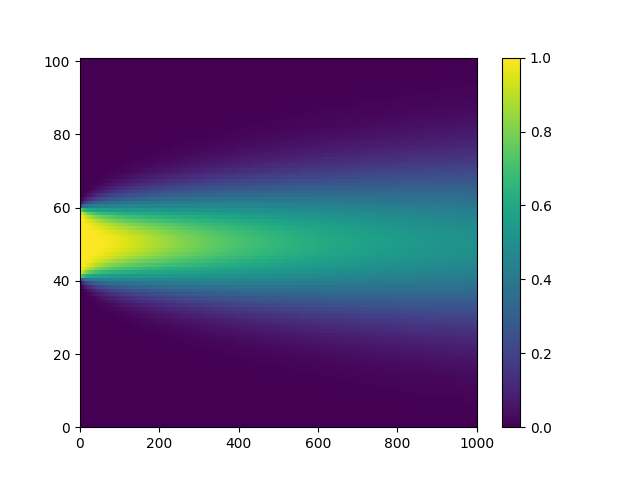
\includegraphics[width=\textwidth]{graficos/difusion-alpha01.png}
            \caption{Heatmap para $\alpha = 0.1$}
            \label{fig:heatmap_alpha_01}
      \end{subfigure}%
      \begin{subfigure}{.5\textwidth}
            \centering
            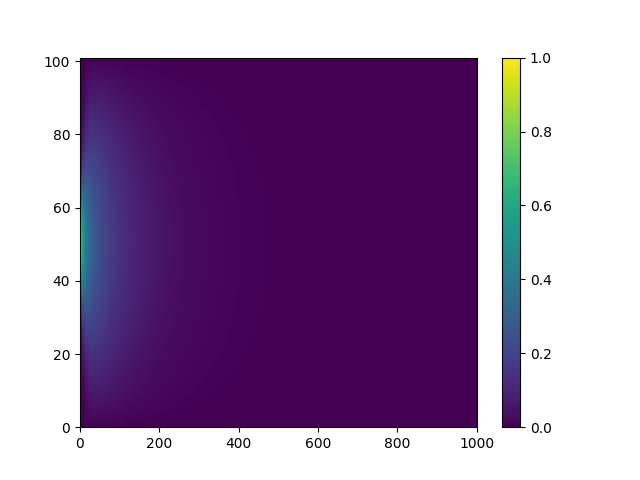
\includegraphics[width=\textwidth]{graficos/difusion-alpha10.png}
            \caption{Heatmap para $\alpha = 10$}
            \label{fig:heatmap_alpha_10}
      \end{subfigure}
      \caption{Heatmap con distintos valores de $\alpha$}
      \label{fig:heatmap_diff_alpha}
\end{figure}

Se puede observar que, mientras que para $\alpha=0.1$ la difusión del valor de los elementos centrales es menor y más lenta, por otro lado para $\alpha = 10$ los valores se dispersan mucho más rápido que en los casos anteriores.

Podemos concluir que $\alpha$ es muy importante al determinar el grado de difusión ya que su variación provoca resultados muy diferentes en la manera en la cual se dispersan los valores.
Para valores de $\alpha$ cercanos a $0$ obtenemos un foco centrado en los datos iniciales y una difusión mas lenta, pero para valores de $\alpha$ superiores a $1$ el foco se dispersa mucho más rápidamente.
%%%%%%%%%%%%%%%%%%%%%%%%%%%%%%%%%%%%%%%%%%%%%%
\section{Conclusiones} \label{sec:Conclusiones}
Los experimentos planteados muestran de manera clara cómo el algoritmo de Eliminación Gaussiana que aprovecha la estructura tridiagonal de las matrices utilizadas reduce notablemente los tiempos de ejecución en comparación a la versión tradicional, pasando de una complejidad computacional cúbica a una complejidad de orden lineal. Por otra parte, también demuestran que esta versión tridiagonal del algoritmo puede optimizarse mediante el precómputo de la diagonalización de la matriz, reduciendo aún más los tiempos de ejecución observados.

En cuanto al cálculo del Laplaciano discreto con los métodos propuestos, los resultados observados fueron los esperados, mostrando nuestra implementación un comportamiento idéntico al presentado por la cátedra.

Por último, se utilizaron los algoritmos desarrollados en el presente trabajo para experimentar la simulación de un proceso de difusión. Se demostró el rol que juega el parámetro $\alpha$ en la velocidad de la difusión de los valores inicialmente concentrados en el centro del vector.

%%%%%%%%%%%%%%%%%%%%%%%%%%%%%%%%%%%%%%%%%%%%%%
\bibliographystyle{plain}
\bibliography{refs}

\end{document}


